\documentclass[onecolumn]{article}
\usepackage[spanish]{babel}
\usepackage{caption}
\usepackage{graphicx}
\usepackage{amsmath}
\setlength{\parindent}{0pt}

\author{Josué Villasante}
\title{Medición del tamaño del haz de un laser}

\begin{document}
	\maketitle

	\section{Objetivo}
		El objetivo fue obtener el tamaño del haz del láser utilizando dos procedimientos. El primer procedimiento consistió en utilizar una cuchilla para medir luego de ella como cambia la intensidad a medida esta va bloqueando el haz. El segundo procedimiento utilizó la camara fotográfica para obtener una imagen de la intesidad del haz.

	\section{Resultados}
		De la imagen capturada por una camara (Thorlabs DCU223C) se tomó la fila que presentó la mayor intensidad y esta se ajustó a una gaussiana. 
		$$
		f(x) = \frac{1}{\sigma\sqrt{2\pi}}\exp({-\frac{(x-\mu)^2}{2\sigma^2}})
		$$
		Esto se puede ver en la imagen \ref{cintura_1}. Los parámetros que se obtuvieron del ajuste fueron $\sigma=45.75$ y $\mu=392.07$. Tomando en cuenta que la altura del sensor son 3.571mm se obtuvo que el diametro del haz utilizando \textit{Full width at half maximum}(FWHM) es 0.50mm y 0.85mm tomando los puntos que son $1/e^2$ veces el máximo.

		\begin{center}
			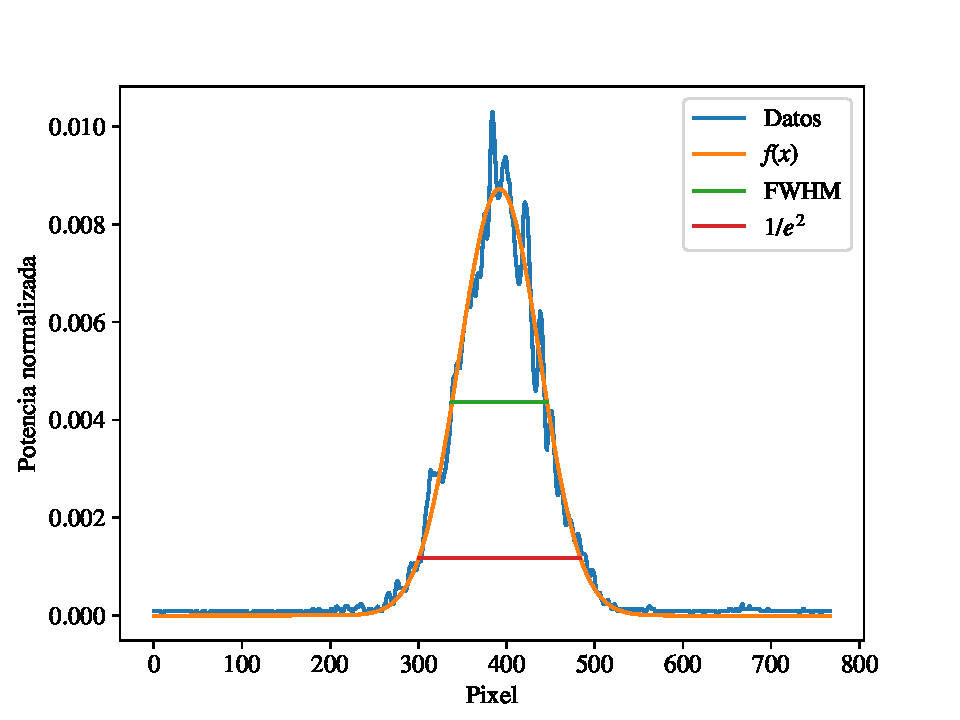
\includegraphics[width=200pt]{img/plot-LaserCintura.pdf}
			\captionof{figure}{Distribución normal ajustada a la potencia normalizada y capturada por una fila de pixeles de la cámara.}
			\label{cintura_1}
		\end{center}

		Lo mismo se realizó para el haz luego de pasar por la fibra. Los parámetros que se obtuvieron del ajuste fueron $\sigma=97.80$ y $\mu=375.89$. El diametro del haz utilizando FWHM fue 1.07mm y 1.81mm tomando los puntos que son $1/e^2$ veces el máximo.

		\begin{center}
			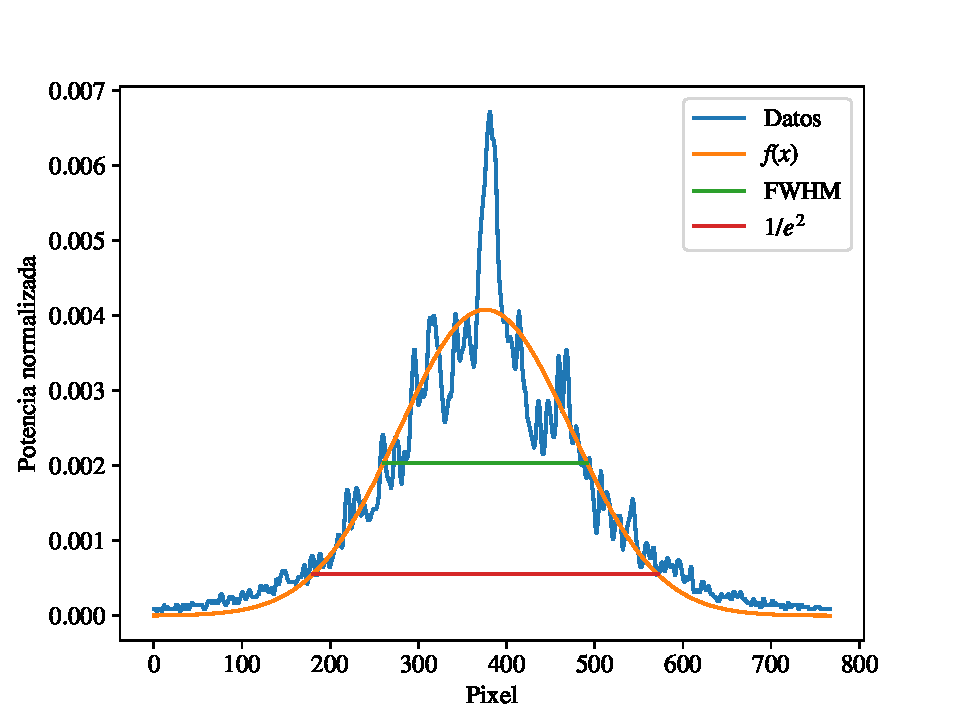
\includegraphics[width=200pt]{img/plot-FibraCintura.pdf}
			\captionof{figure}{Distribución normal ajustada a la potencia normalizada y capturada por una fila de pixeles de la cámara.}
			\label{cintura_2}
		\end{center}
	
	\section{Diametro del haz en el punto focal de un lente}
		\subsection{Marco teórico}
		Luego de que un haz Gaussiano pasa por un lente, este se reduce en tamaño hasta llegar al punto mínimo en el punto focal. En el punto focal el tamaño del haz es descrito por
		$$
			w_f=\frac{\lambda f}{\pi w_0}
		$$
		donde $w_f$ es el tamaño del haz en el punto focal, $\lambda$ es la longitud de onda, $f$ es la distancia focal y $w_0$ es el tamaño inicial del haz (antes del lente).

		Sin embargo, existen imperfecciones en el lente por lo cual no se obtiene un haz Gaussiano ideal. Esto es modelado usualmente agregando un parámetro $M^2$ que representa el factor de calidad.
		\begin{equation}
			w_f=\frac{M^2 \lambda f}{\pi w_0}
		\label{focal_width}
		\end{equation}

		Utilizando el tamaño del haz en el punto focal podemos obtener también la distancia de Rayleigh $z_R$. Esta indica la distancia alrededor del punto focal donde el haz se mantiene relativamente coalimado.
		$$
			z_R=\frac{\pi w_f^2}{\lambda}
		$$

		Finalmente, el tamaño del haz puede ser descrito por
		\begin{equation}
			w(z)=w_f \sqrt{1+\left(\frac{z}{z_{\mathrm{R}}}\right)^2}
		\label{beamwidth}
		\end{equation}
		donde $w_f$ corresponde al diámetro del haz punto focal y $z_R$ a la distancia de Rayleigh.

		\subsection{Procedimiento y resultados}
		El objetivo inicial fue obtener el tamaño del haz en varios puntos luego de pasar por un lente. Se realizó el siguiente arreglo experimental (fig. \ref{arreglo_dist_focal}), dónde se realizaron 13 fotografías. Por cada una la distancia entre el lente y la camara se redujo en 5 mm. Se empezó a fotografiar a 11.5 cm del lente.

		\begin{center}
			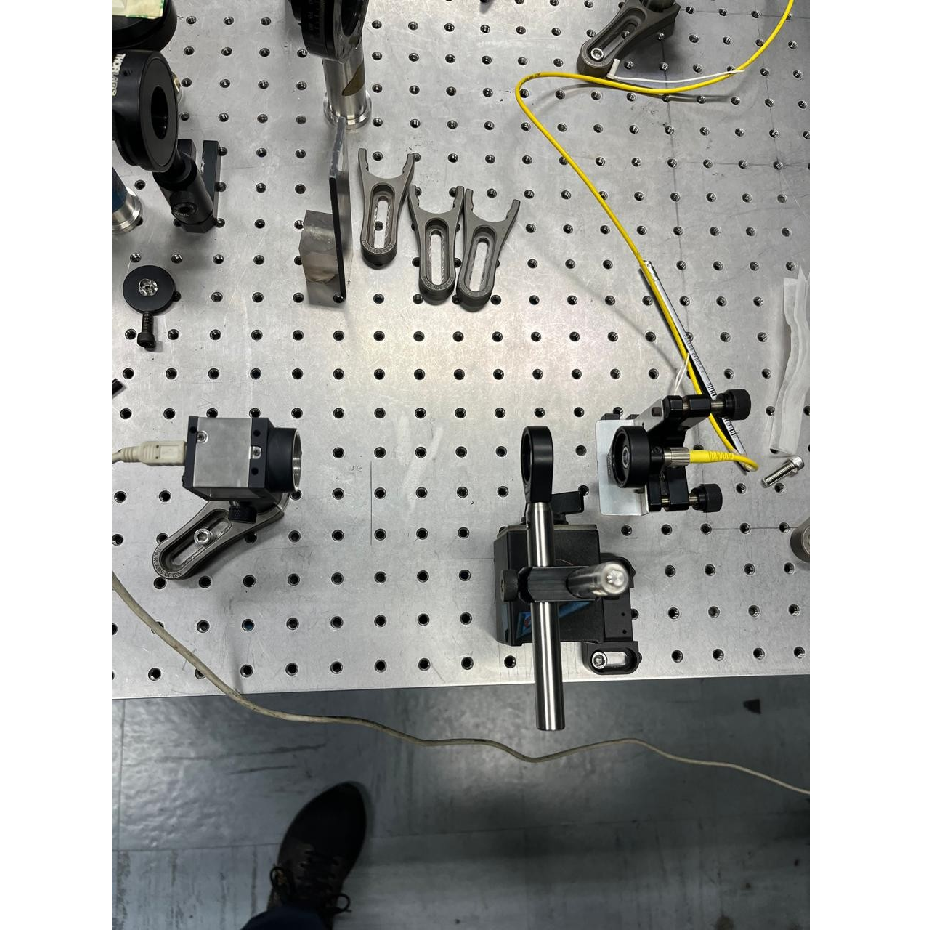
\includegraphics[width=150pt]{img/dist_focal/arreglo.pdf}
			\captionof{figure}{Arreglo experimental utilizado para medir la distancia focal.}
			\label{arreglo_dist_focal}
		\end{center}

		La siguiente imagen (fig. \ref{ejemplo_image_capturada}) es un ejemplo de las 13. Por cada una de ellas se ajustó una distribución normal a la fila más intensa hallando un valor para $\sigma$.
		\begin{center}
			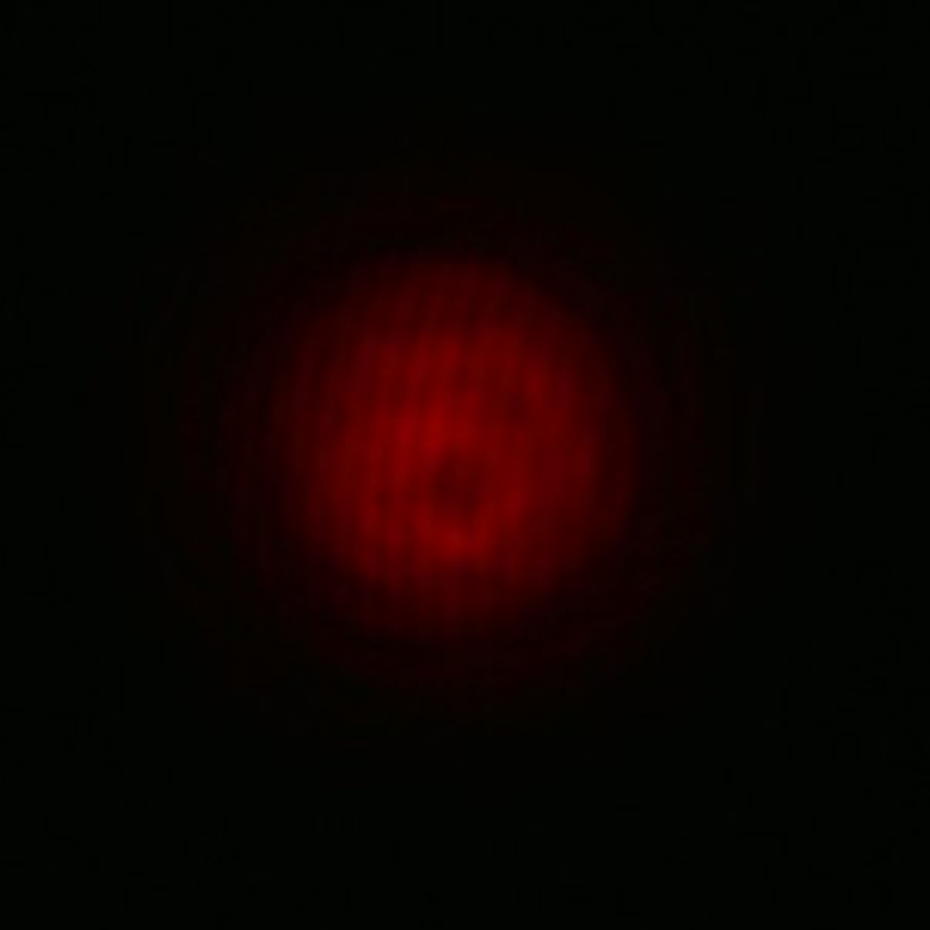
\includegraphics[width=100pt]{img/dist_focal/image_sample.pdf}
			\captionof{figure}{Ejemplo de imagen capturada.}
			\label{ejemplo_image_capturada}
		\end{center}

		\begin{center}
			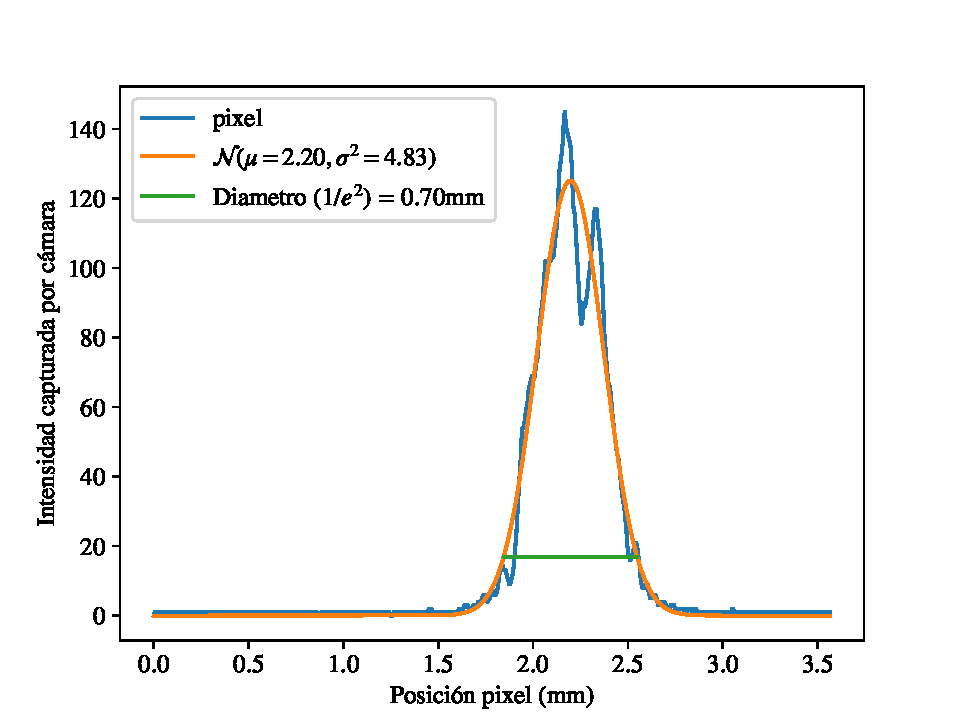
\includegraphics[width=300pt]{img/dist_focal/plot_sample.pdf}
			\captionof{figure}{Ejemplo de imagen capturada y ajuste realizado.}
			\label{ejemplo_ajuste}
		\end{center}

		Una vez calculados todos los diámetros estos se graficaron (fig. \ref{focal_point}) en funcion de la distancia del lente a la cámara. A estos puntos se hizo un ajuste de la función \ref{beamwidth} y se obtuvo un valor para el diámetro del haz en el punto focal, $w_f=0.0389 mm$ y la distancia de Rayleigh, $z_R=0.1995$. Calculando el punto mínimo de la función se puede obtener que la distancia focal es de 8.06 mm.

		\begin{center}
			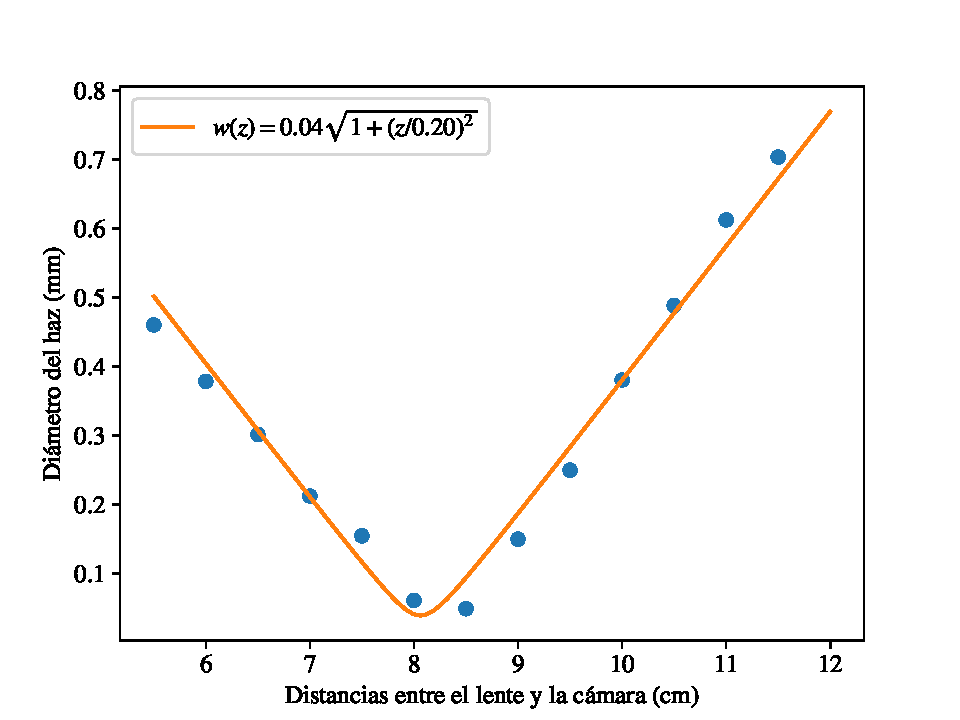
\includegraphics[width=300pt]{img/dist_focal/focal_point.pdf}
			\captionof{figure}{Diámetro del haz en función de la distancia.}
			\label{focal_point}
		\end{center}

		Por otro lado, también podemos obtener un valor para el ancho del haz utilizando la ecuación \ref{focal_width} y tomando en cuenta que estamos trabajando con un laser modelo ThorLabs HNL100L. Este tiene una longitud de onda de 632.8 nm y un factor de calidad ($M^2$) de 4.05. Obtenemos que $w_f=0.0362 mm$, lo cual corresponde con lo obtenido anteriormente.

	\section{Interferómetro}
	\subsection{Marco teórico}
		Un haz polarizado horizontalmente puede ser representado de manera vectorial.
		$$
		|H\rangle=\binom{1}{0}
		$$
		Sobre este pueden actuar elemento ópticos como son laminas retardadoras. En el formalismo de Jones vemos que las laminas de media onda y cuarto de onda sin rotación pueden ser representadas por
		$$
		\hat{W}_{\lambda / 2}=\left(\begin{array}{cc}
		1 & 0 \\
		0 & -1
		\end{array}\right)
		$$
		$$
		\hat{W}_{\lambda / 4}=\left(\begin{array}{ll}
		1 & 0 \\
		0 & i
		\end{array}\right)
		$$
		Utilizando la matriz de rotación podemos incluir la rotación de la lamina retardadora y obtenemos representaciones para la lamina de media y cuarto de onda.
		$$
		\hat{W}_{\lambda / 2}(\theta)=\hat{R}(\theta) \hat{W}_{\lambda / 2} \hat{R}(-\theta)
		$$
		$$
		\hat{W}_{\lambda / 4}(\theta)=\hat{R}(\theta) \hat{W}_{\lambda / 4} \hat{R}(-\theta)
		$$

		Luego para obtener una probabilidad (que será proporcional a la intensidad) representamos matricialmente el polarizador por
		$$
		\hat{P}_H=|H\rangle\langle H|=
		\left(\begin{array}{ll}
		1 & 0 \\
		0 & 0
		\end{array}\right)
		$$
		$$
		\mathcal{P}_X=|\hat{P}_X | \psi_f\rangle|^ 2
		$$
		Utilizando este formalismo podemos armar un arreglo y observar si se presenta o no un patrón de interferencia, y observar si se presenta una variación en visibilidad, $\nu$, en función de los ángulos de la lamina.
		$$
		\nu=\frac{I_{\max }-I_{\min }}{I_{\max }+I_{\min }}
		$$
	\subsection{Procedimiento y resultados}
		Para observar los diferentes comportamientos de la visibilidad realizamos el siguiente arreglo experimental. Primero utilizó un polarizing beam splitter para preparar un haz de polarización horizontal. Luego el haz pasó por 3 laminas retardadoras, para luego pasar por un polarizador y fue detectado por un potenciómetro. El juego de 3 laminas las llamaremos H1, H2 y H3, dónde H3 es el más cercano al detector.
		\begin{center}
			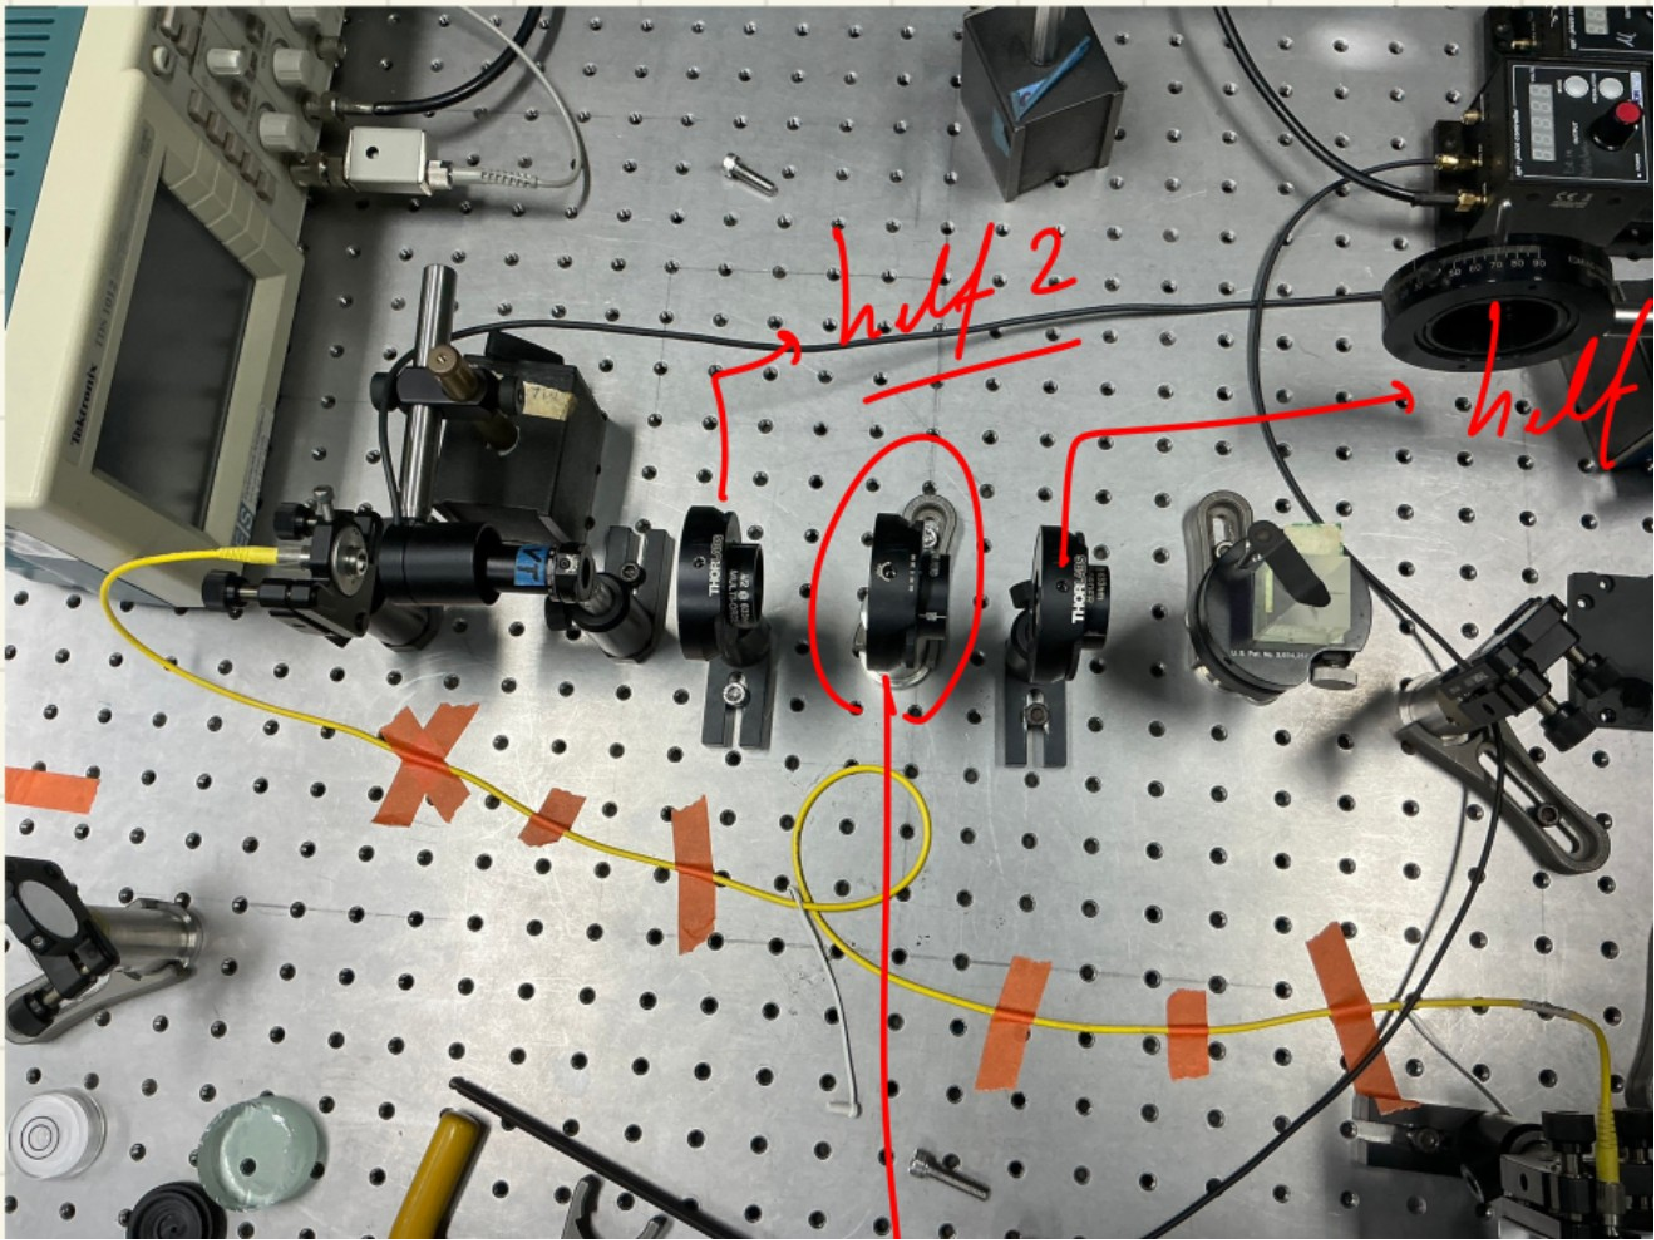
\includegraphics[width=150pt]{img/inter/arreglo.pdf}
			\captionof{figure}{Arreglo experimental.}
			\label{inter_arreglo}
		\end{center}

		Lo que varió en el experimento fue el elemento óptico que se colocó en H2. Inicialmente, para observar un primer patrón no se colocó nada, y se variaron los ángulos de H1 y H2, donde el ángulo de H1 fue el negativo de H2. Este patrón es representado por $\phi=0$ en la figura \ref{super_vis}. Luego se realizó lo mismo pero colocando una lamina $\lambda/2$ en H2, y se obtuvo el patrón de $\phi=\pi$. Finalmente se colocó una lamina $\lambda/4$ en H2 y se obtuvo el patrón restante.
		
		\begin{center}
			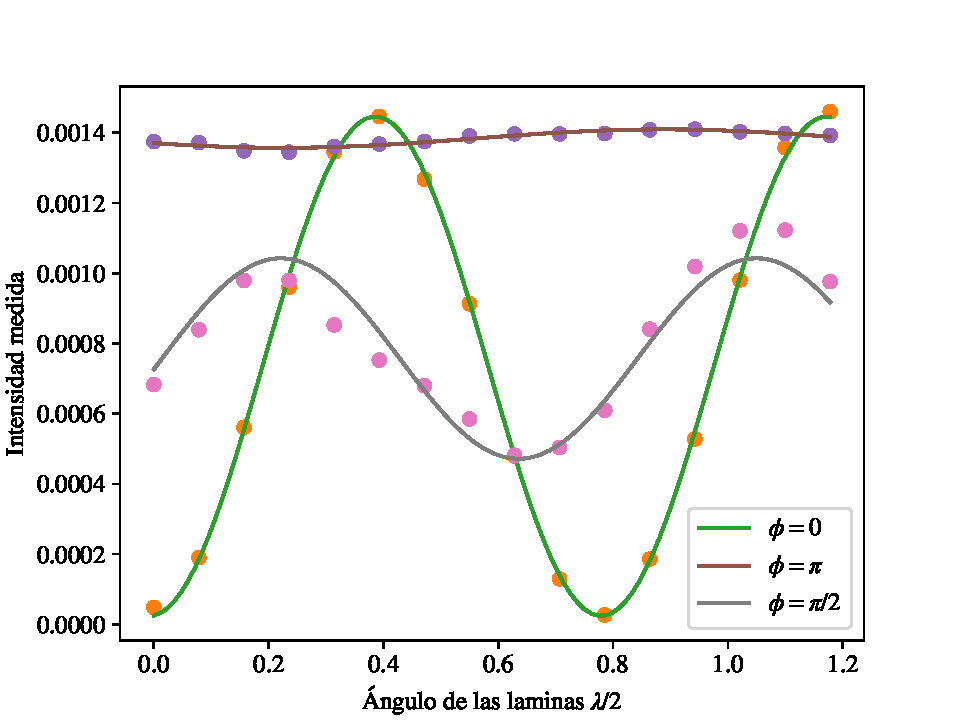
\includegraphics[width=200pt]{img/inter/super_vis.pdf}
			\captionof{figure}{Patrón de intensidad para tres elementos en H2.}
			\label{super_vis}
		\end{center}

		Para el caso donde H2 está vació podemos respresentar el estado final del arreglo como
		$$
		| \psi_f\rangle=\hat{W}_{\lambda / 2}(-\theta)\hat{W}_{\lambda / 2}(\theta)|H\rangle
		$$
		La probabilidad de obtener una medición la podemos representar como
		$$
		\mathcal{P}_X=|\hat{P}_X | \psi_f\rangle|^ 2=\left|8 \sin ^4(\theta)-8 \sin ^2(\theta)+1\right|^2
		$$
		que es justamente un patrón de interferencia mostrado en la medición.
		
		Para el caso donde H2 es una lamina $\lambda/2$ podemos realizar la misma operación incluyendo esta nueva operación.
		$$
		| \psi_f\rangle=\hat{W}_{\lambda / 2}(-\theta)\hat{W}_{\lambda / 2}(0)\hat{W}_{\lambda / 2}(\theta)|H\rangle
		$$
		Operando obtenemos que la probabilidad de obtener una medición es constante, que es lo que vimos en el resultado de la figura \ref{super_vis}.
		$$
		\mathcal{P}_X=|\hat{P}_X | \psi_f\rangle|^ 2=1
		$$

		Finalmente para el caso donde H2 es una lamina $\lambda/4$, tenemos que
		$$
		| \psi_f\rangle=\hat{W}_{\lambda / 2}(-\theta)\hat{W}_{\lambda / 4}(0)\hat{W}_{\lambda / 2}(\theta)|H\rangle
		$$
		y operando obtenemos una expresión más compleja pero que igual muestra un patrón  de interferencia.
		$$
		\mathcal{P}_X=|\hat{P}_X | \psi_f\rangle|^ 2=\frac{\left|i(\cos (4 \theta)-1)+2 \cos ^2(2 \theta)\right|^2}{4}
		$$

		Para este último caso si tomamos en cuenta que el ángulo de la lamina $\lambda/4$ puede ser cualquier angulo obtenemos
		$$
		| \psi_f\rangle=\hat{W}_{\lambda / 2}(-\theta)\hat{W}_{\lambda / 4}(\alpha)\hat{W}_{\lambda / 2}(\theta)|H\rangle
		$$
		$$
		\mathcal{P}_X=|\hat{P}_X | \psi_f\rangle|^ 2=\left|(1-i) \sin ^2(\alpha)-4 \cdot(1+i) \sin ^4(\theta)+4 \cdot(1+i) \sin ^2(\theta)-1\right|^2
		$$
		donde observamos que $\alpha$ no afecta la diferencia $I_{\max }-I_{\min }$ por lo que la visibilidad se debe mantener igual para cualquier valor de $\alpha$. Esto fue lo que realizamos experimentalmente para 5 valores de $\alpha$ (fig. \ref{super_qwp}).
		\begin{center}
			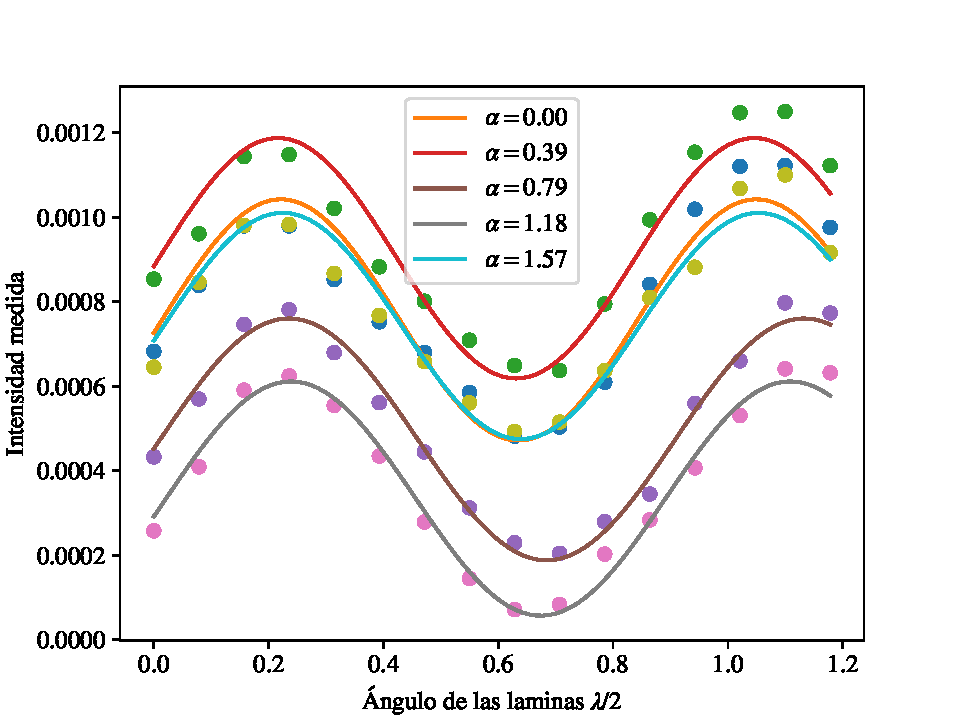
\includegraphics[width=200pt]{img/inter/super_qwp.pdf}
			\captionof{figure}{Patrón de intensidad para distintos valores de $\alpha$.}
			\label{super_qwp}
		\end{center}
\end{document}